Para concluir los aspectos generales que debe cumplir la aplicación, se realiza un estudio para comprender la situación actual de un proceso de solicitud de fondos por rendir. Si bien existen varias OE, esta memoria se enfoca en dos de ellas, a saber, Federación (de estudiantes del campus Curicó) y CCAA tal como se menciona en la \textbf{Sección \ref{sec:Contexto}}. Al realizar el estudio, se lleva a cabo un diagrama que explica el proceso que conlleva solicitar un fondo por rendir por parte de Federación (ver \textbf{Figura \ref{fig: Solicitud_Federacion}}) y el proceso que deben realizar los CCAA (ver \textbf{Figura \ref{fig: Solicitud_CAA}}).

\begin{figure}[tb!]
    \hspace{-9mm}
    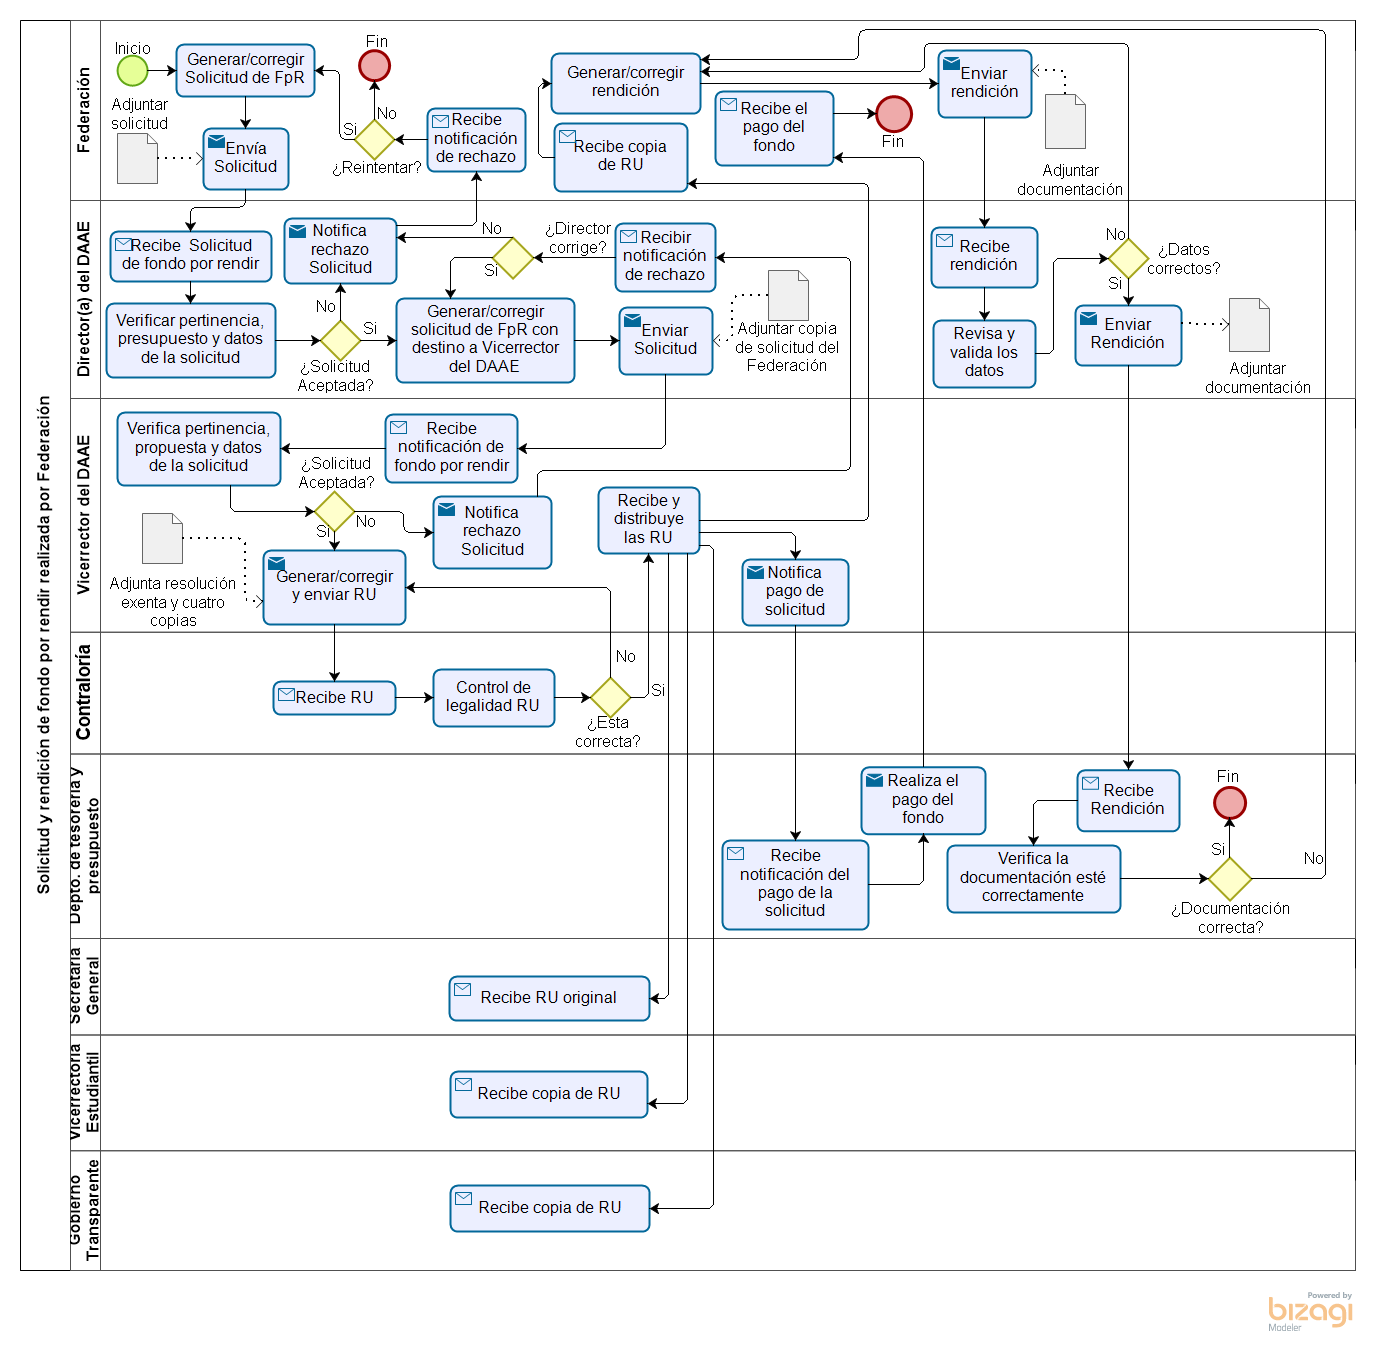
\includegraphics[width=1.1\textwidth]{Imagenes/Solicitud_Federacion_Rendicion.png}
    \caption{\label{fig: Solicitud_Federacion}Proceso de Fondos por Rendir por parte de Fedeut.}
\end{figure}

El proceso que conlleva la solicitud de un Fondo por Rendir por parte de Federación que representa la \textbf{Figura \ref{fig: Solicitud_Federacion}} es:

\begin{enumerate}
    \item Elevar una solicitud a la DAAE. 
    \item Si se acepta la solicitud de Federación por parte la DAAE, este debe elevar una solicitud a quien dirige la Vicerrectoría de la DAAE junto con una copia de la solicitud realizada por Federación. 
    \item En caso de ser aceptada la solicitud por parte de la Vicerrectoría de la DAAE, esta crea la RU de aprobación de la Solicitud junto con tres copias para luego ser enviada al departamento de Contraloría el cual se encarga de chequear que el documento esté correctamente realizado. 
    \item En caso de ser aprobado por Contraloría, se envían nuevamente a Vicerrectoría de la DAAE y luego se procede a distribuir los documentos quedando el original en Secretaría General, y las cuatro copias son distribuidas a la OE interesada, al Gobierno Trasparente, al Departamento de Tesorería y Presupuesto y a la Vicerrectoría Estudiantil.
    \item Tras ser aprobada la solicitud y enviada la RU a los departamentos, Tesoreria genera un Cheque al nombre del responsable del evento y lo envia a Federación.
    \item Tras recibir la RU por parte de Federación, este se encarga de realizar el evento y después comenzar con el proceso de Rendición de la actividad. 
    \item Una vez finalizada la Rendición, se envía a quien dirige la DAAE y en caso de ser aprobada se envía la Rendición al departamento de Tesorería y Presupuesto para su posterior revisión.
    \item En caso de ser aprobada, se finaliza el proceso de Solicitud de Fondo por Rendir, en caso contrario, se envía a la OE que realizó la Rendición para ser corregida e iniciar por el proceso de revisión nuevamente hasta cuando sea aprobada.
\end{enumerate}

\begin{figure}[tb!]
    \hspace{-9mm}
    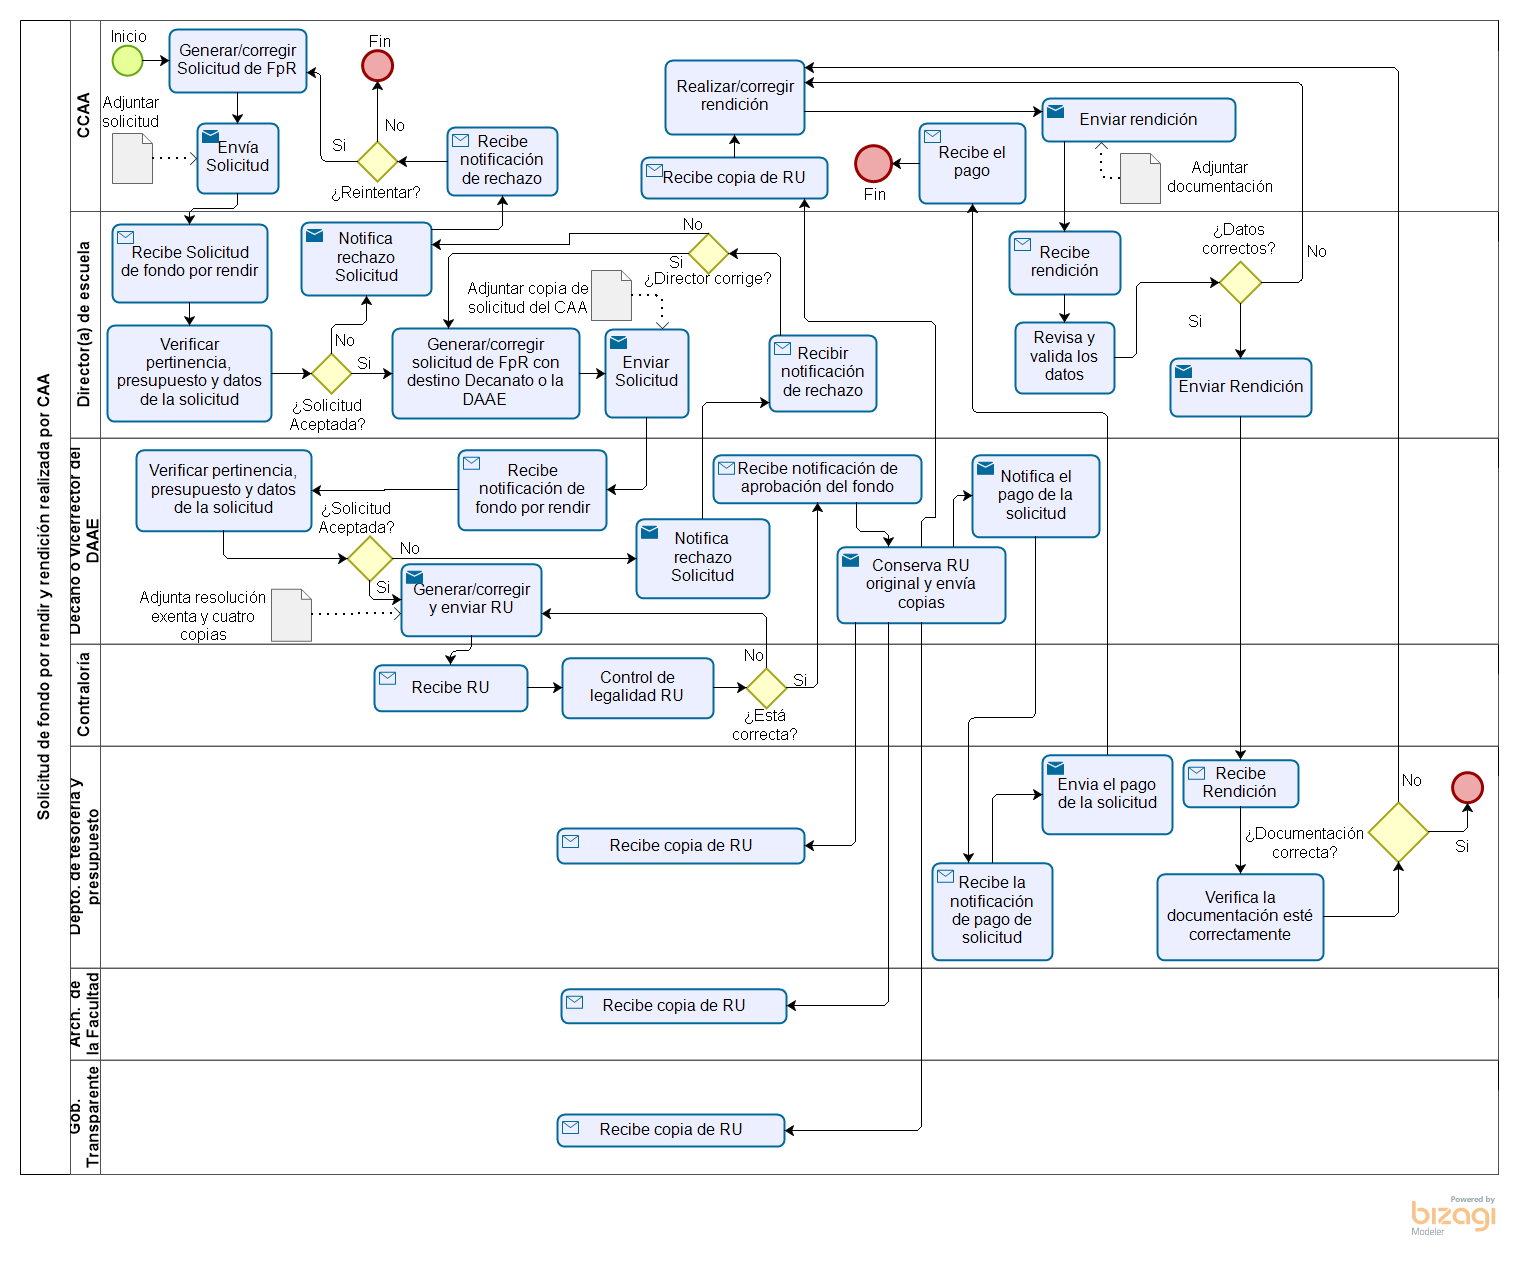
\includegraphics[width=1.1\textwidth]{Imagenes/Solicitud_CCAA_Rendicion.png}
    \caption{\label{fig: Solicitud_CAA}Proceso fondos por rendir por parte de un CAA.}
\end{figure}

El proceso que conlleva la solicitud de un Fondo por Rendir por parte de los CCAA que representa la \textbf{Figura \ref{fig: Solicitud_CAA}} es:

\begin{enumerate}
    \item Elevar una solicitud al Director(a) de Escuela de su respectiva Carrera. 
    \item Si se acepta la solicitud del CAA por parte de la Dirección de la Escuela, esta debe elevar una solicitud a Decanato junto con una copia de la solicitud realizada por el CAA. 
    \item En caso de ser aceptada la solicitud por parte de Decanato, este crea la RU de aprobación de la Solicitud junto con cuatro copias para luego ser enviada al departamento de Contraloría, quien se encarga de chequear que el documento esté correctamente realizado. 
    \item En caso de ser aprobado por Contraloría, se envían nuevamente a Decanato y luego se procede a distribuir los documentos quedando el original en Decanato, y las cuatro copias son enviadas a la OE interesada, al departamento de Tesorería y Presupuesto, al Archivo de la Facultad y Gobierno Trasparente.
    \item Tras ser aprobada la solicitud y enviada la RU a los departamentos Tesoreria genera un Cheque al nombre del responsable del evento y lo envia a la Escuela de la cual proviene la solicitud para ser entregada al respectivo CAA.
    \item Tras recibir la RU por parte del CAA, este se encarga de realizar el evento y después comenzar con el proceso de Rendición de la actividad. 
    \item Una vez finalizada la Rendición, se envía a la Dirección de la Escuela y en caso de ser aprobada se envía la Rendición al departamento de Tesorería y Presupuesto para su posterior revisión.
    \item En caso de ser aprobada, se finaliza el proceso de Solicitud de Fondo por Rendir, en caso contrario, se envía a la OE que realizó la Rendición para ser corregida e iniciar por el proceso de revisión nuevamente hasta cuando sea aprobada.
\end{enumerate}


Tal como se aprecia, ambos procesos son similares. En el \textbf{Cuadro \ref{tab: tab_dif_proc_FpR}} se muestran las diferencias.

\begin{table}[htbp]
    
    \caption{\label{tab: tab_dif_proc_FpR} Diferencia en el proceso de Fondos por Rendir entre Fedeut y CCAA. }
    \footnotesize
    \begin{tabular}{|p{7.1cm}|p{7.1cm}|}
    
    \hline
    \textbf{Fedeut} & \textbf{CCAA} \\
    
    \hline\hline
    
    La solicitud de fondos va dirigida a la DAAE. & La solicitud de fondos va dirigida a la Dirección de Escuela.\\ \hline

    La solicitud de la DAAE junto con la solicitud de Federación va dirigida al Vicerrectoría de la DAAE. & La solicitud de la Dirección de Escuela junto con la solicitud del CCAA va dirigido a Decanato.\\ \hline

    La RU original queda en el archivo de Secretaría General. & La RU original queda en Decanato.\\ \hline

    \end{tabular}  
\end{table}

Por su parte, tanto Federación como los CCAA deben cumplir con lo siguiente:

\begin{itemize}
    \item Ambas OE deben confeccionar una solicitud para inicializar el proceso de fondos por rendir (ver \textbf{Sección \ref{sec:Conceptos}}).
    \item En caso de que la solicitud es aprobada, las OE deben recibir una copia de la RU que aprueba la solicitud.
    \item Tras obtenida la RU que acredita la aprobación de la solicitud de un fondo por rendir y realizado el evento por el cual se solicita el fondo, se debe confeccionar la rendición de la actividad (ver \textbf{Sección \ref{sec:Conceptos}}).
\end{itemize}

Dado a lo mencionado anteriormente es que se realiza un diagrama de estado, el cual representa el proceso que realiza las OE y por lo tanto el proceso que debe simular la aplicación (ver \textbf{Figura \ref{fig: diagrama_estado}}).

\begin{figure}[h!tb]
    \hspace{-9mm}
    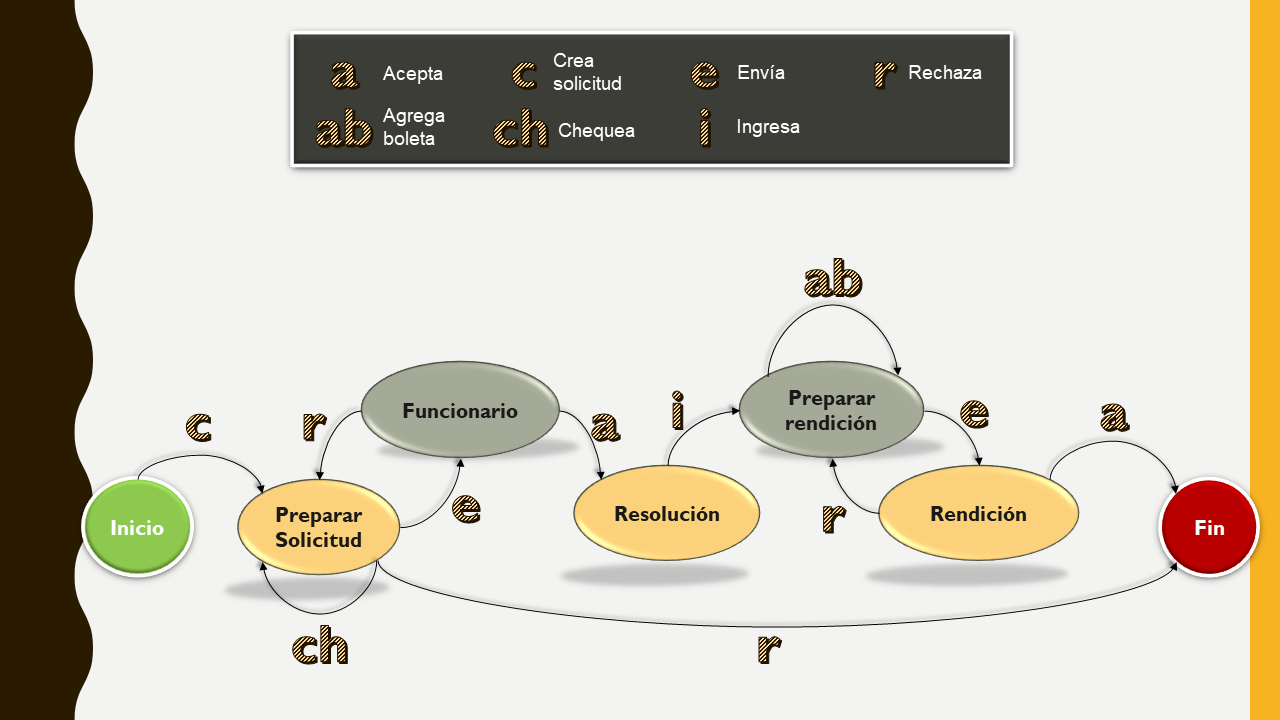
\includegraphics[width=1.1\textwidth]{Imagenes/Diagrama_de_estado.png}
    \caption{\label{fig: diagrama_estado}Diagrama de estado del proceso que debe simular la aplicación.}
\end{figure}

El diagrama de estado que se observa en la \textbf{Figura \ref{fig: diagrama_estado}} muestra las actividades que son de responsabilidad exclusiva de la OE, las cuales son la confección de la Solicitud, la recepción de la Resolución emitida por la Universidad y la posterior Rendición del fondo presupestado. El resto de las actividades que se muestran en las \textbf{Figuras \ref{fig: Solicitud_Federacion}} y \textbf{\ref{fig: Solicitud_CAA}} son realizadas por las demás entidades involucradas en el proceso.

A grandes rasgos, el sistema emula el proceso de una Solicitud de Fondo por Rendir desde el punto de vista de la OE. Este proceso conlleva la confección de una Solicitud y su exportación en formato PDF. En caso que la solicitud sea aceptada, la OE recibe la RU respectiva enviada por parte de la Casa de Estudio. Luego, la OE almacena en el sistema una copia digitalizada de la RU respectiva en formato PDF. Por último, la OE debe confeccionar la Rendición de los gastos efectuados durante el evento y su posterior exportación en formato PDF.


Cabe destacar que no es el único proceso en el cual las OEs realizan declaraciones de gastos. Existe otra forma en la se puede solicitar un Fondo pero con Solicitud de reembolso para las distintas OEs y que se pueden apreciar en las \textbf{Figuras \ref{fig: Solicitud_CAA_Reembolso}} y \textbf{\ref{fig: Solicitud_Federacion_Reembolso}}. Es por ello que en el  \textbf{Cuadro \ref{tab: tab_dif_proc_FpR_FcSR}} se muestran las diferencias entre un Fondo por Rendir y un Fondo con Solicitud de Reembolso.

\begin{figure}[tb!]
    \hspace{-9mm}
    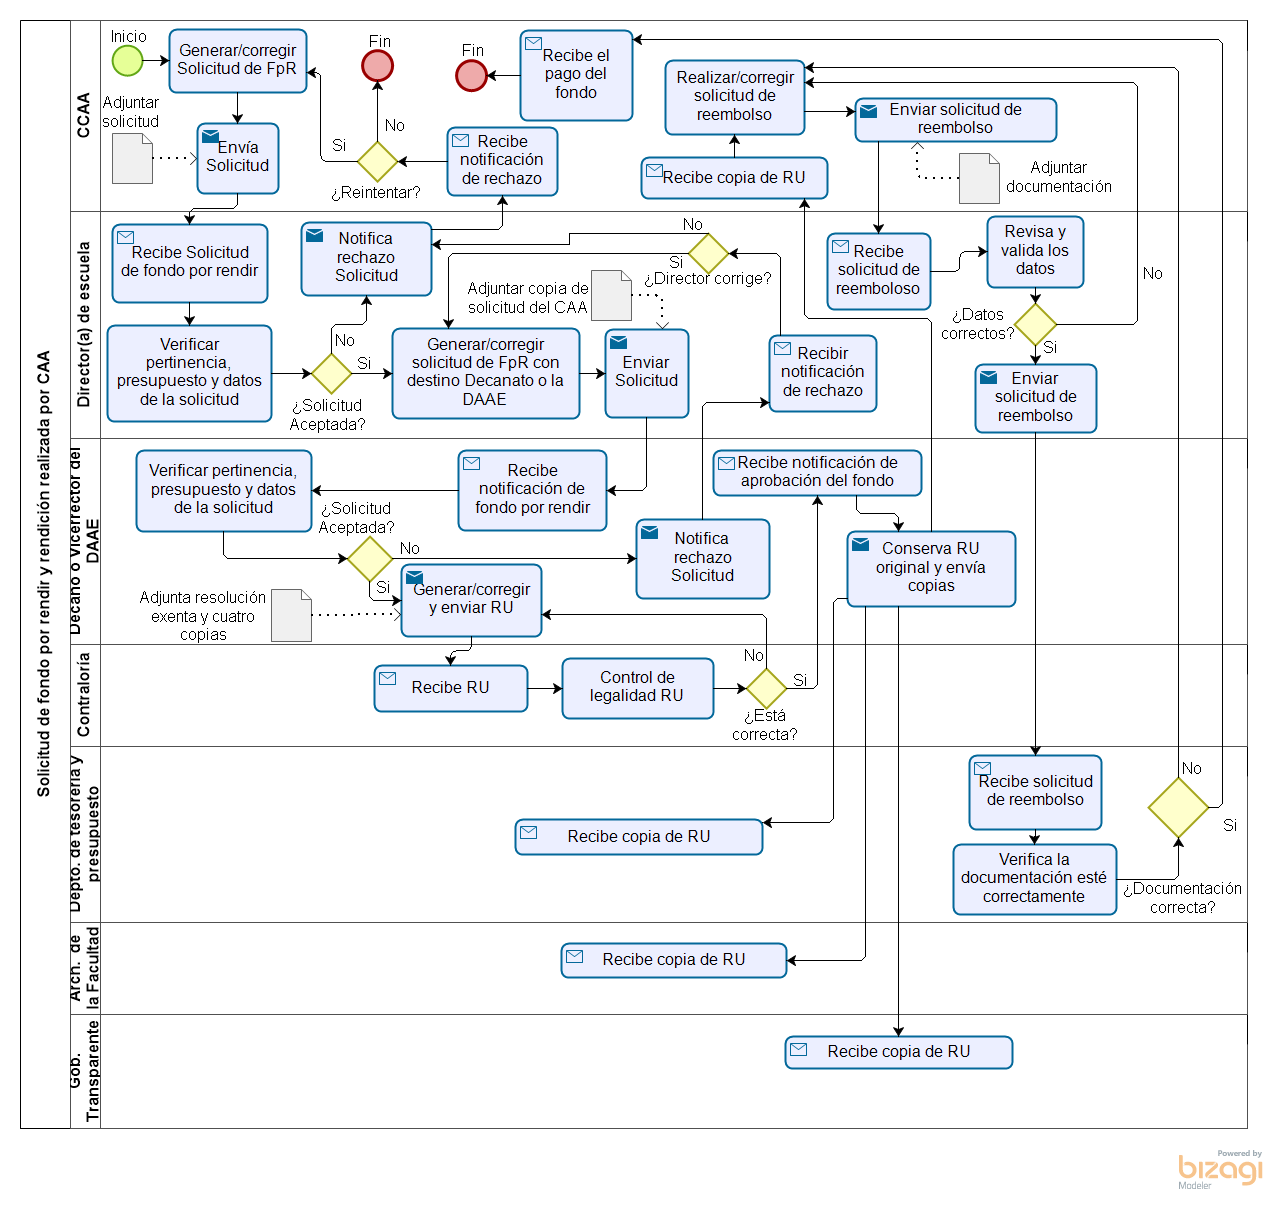
\includegraphics[width=1.1\textwidth]{Imagenes/Solicitud_CCAA_Reembolso.png}
    \caption{\label{fig: Solicitud_CAA_Reembolso}Proceso fondos con Solicirud de Reembolso por parte de un CAA.}
\end{figure}

\begin{figure}[tb!]
    \hspace{-9mm}
    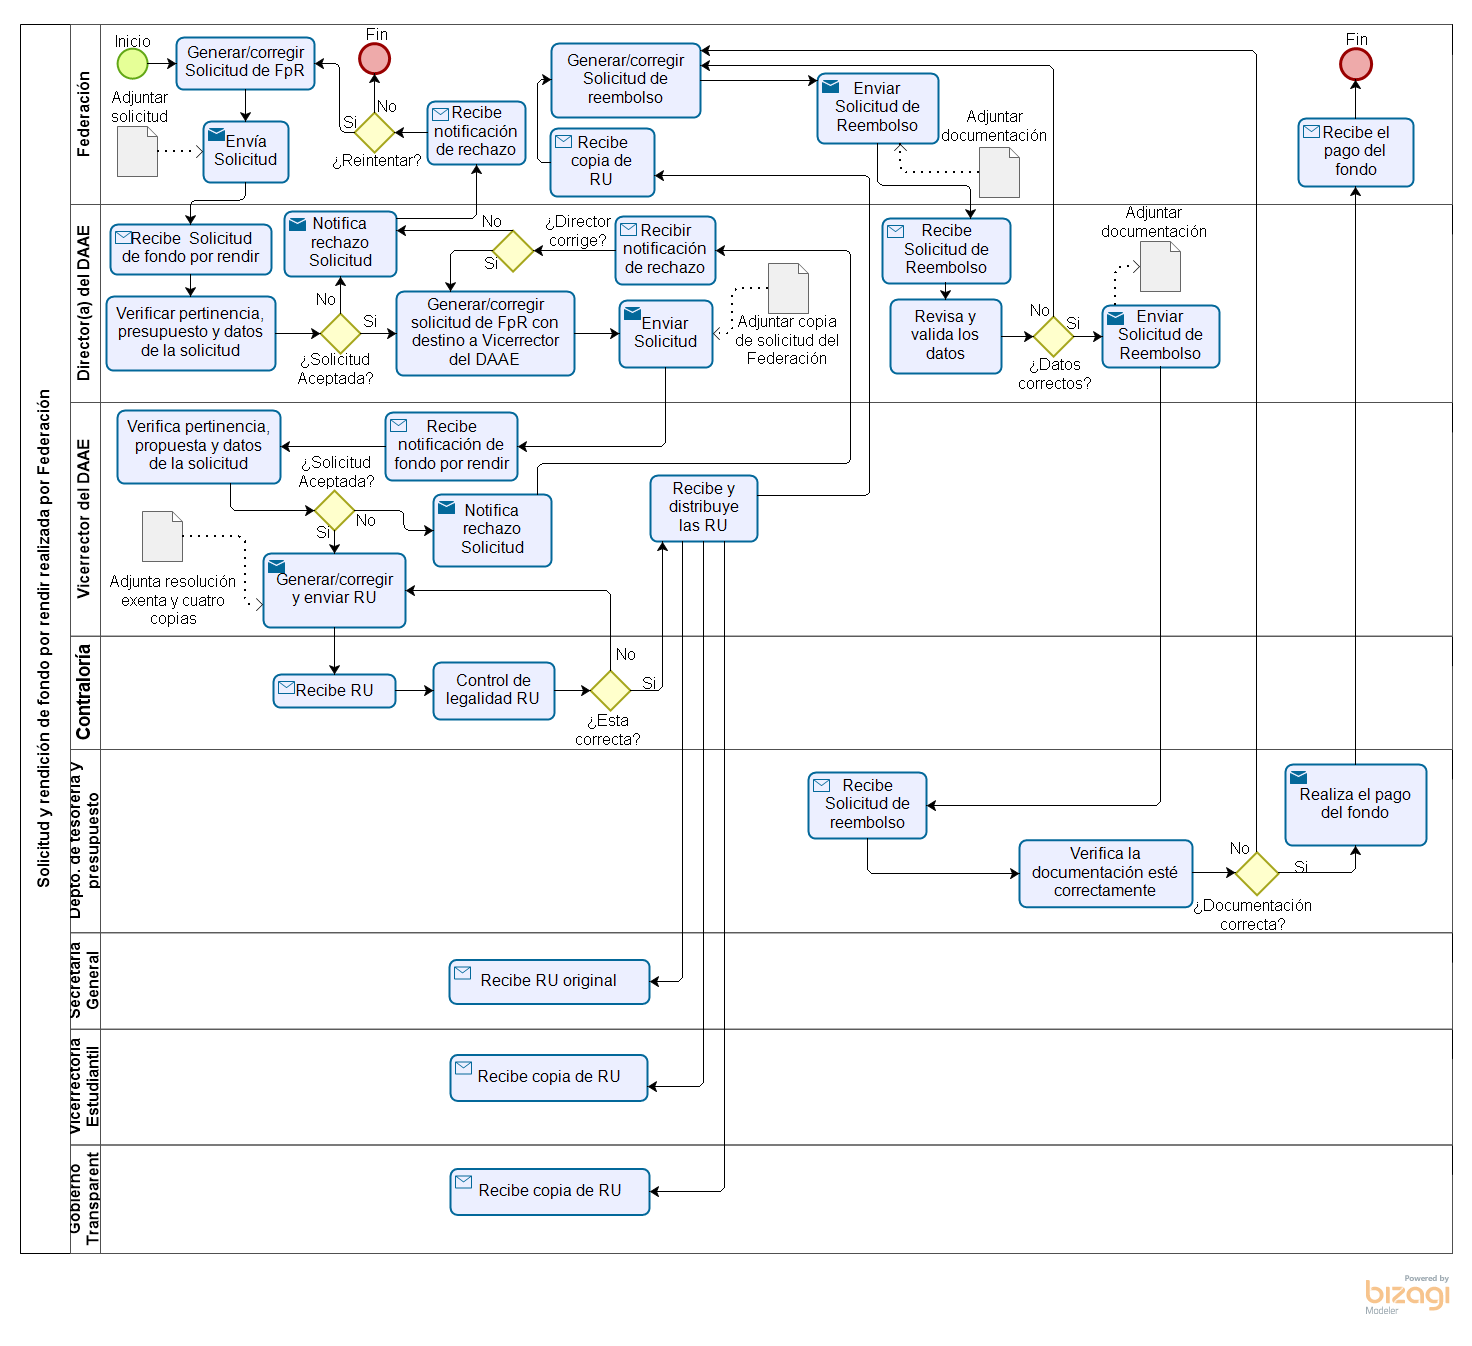
\includegraphics[width=1.1\textwidth]{Imagenes/Solicitud_Federacion_Reembolso.png}
    \caption{\label{fig: Solicitud_Federacion_Reembolso}Proceso fondos con Solicitud de Reembolso por parte de Federación.}
\end{figure}

\begin{table}[htbp]
    
    \caption{\label{tab: tab_dif_proc_FpR_FcSR} Diferencia en el proceso de Fondos por Rendir entre Fedeut y CCAA. }
    \footnotesize
    \begin{tabular}{|p{7.1cm}|p{7.1cm}|}
    
    \hline
    \textbf{Fondo por Rendir} & \textbf{Fondo con Solicitud de Reembolso} \\
    
    \hline\hline
    
    En caso de ser aprobada la Solicitud, el dinero solicitado llega antes de realizar el evento. & En caso de ser aprobada la Solicitud, la OE debe financiar los gastos al momento de realizar el evento.\\ \hline

    Una vez terminada la actividad, se genera el documento en que se declaran los gastos realizado en el evento al cual se le denomina Rendición. & Una vez termiana la actividad, se genera el documento que se declaran los gatos realizados en el evento, pero en este proceso se le denomina Solicitud de Reembolso.\\ \hline

    En caso de que en el evento se haya gastastado menos de lo presupuestado, se debe devolver el dinero restante a la casa de estudios. & En caso de que en el evento haya gastado menos de lo presupuestado, la Universidad reembolsa el dinero efectivamente gastado.\\ \hline

    \end{tabular}  
\end{table}